\documentclass{beamer}
\usetheme{Warsaw}

\usepackage{xcolor}
\usepackage{listings}
\usepackage{textcomp}
\usepackage{ulem}
\usepackage{listings}

\title{Precise GC Support in LLVM}
\author{Ramkumar Ramachandra}
\titlegraphic{
\includegraphics[scale=0.20]{llvm-logo}}

\lstset{
    inputencoding=utf8,
%    backgroundcolor=\color{white},
    tabsize=4,
    rulecolor=,
    numbers=left,
    upquote=true,
%    aboveskip={1.5\baselineskip},
    columns=fixed,
    showstringspaces=false,
    extendedchars=true,
    breaklines=true,
    prebreak = \raisebox{0ex}[0ex][0ex]{\ensuremath{\hookleftarrow}},
    frame=single,
    showtabs=false,
    showspaces=false,
    showstringspaces=false,
    basicstyle=\scriptsize\ttfamily,
    identifierstyle=\ttfamily,
    keywordstyle=[1]\ttfamily\color{blue},
    keywordstyle=[2]\ttfamily\color{purple},
    keywordstyle=[3]\ttfamily\colorbox{yellow},
    commentstyle=\ttfamily\color[rgb]{0.133,0.545,0.133},
    stringstyle=\ttfamily\color[rgb]{0.627,0.126,0.941},
}

\begin{document}

\begin{frame}
  \titlepage
\end{frame}

\begin{frame}{top runtimes}
  \begin{itemize}
  \item[] js: V8/ JSCore/ SpiderMonkey.
  \item[] java, clj, scala: Zing/ Hostspot.
  \item[] rb: MRI/ JRuby.
  \item[] hs: GHC.
  \item[] android: Dalvik/ ART.
  \end{itemize}
  \vfill
  AOT or JIT, everything uses a GC.
\end{frame}

\begin{frame}{users of llvm}
  \begin{itemize}
  \item[] clang (c/c++)
  \item[] opencl
  \item[] julia
  \item[] rust
  \item[] jscore/ftl (new)
  \item[] zing (?)
  \end{itemize}
  \vfill
  llvm needs proper gc support for future adoption.
\end{frame}

\begin{frame}{gc essentials}
  \begin{center}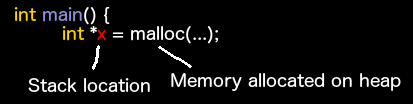
\includegraphics[scale=0.6]{memory-stack-heap}\end{center}
  \vfill
  When the program inevitably loses handles on heap data, the gc kicks
  in to clean up the detritus.
\end{frame}

\begin{frame}{components of a gc}
  \begin{columns}
    \begin{column}[b]{4.5cm}
      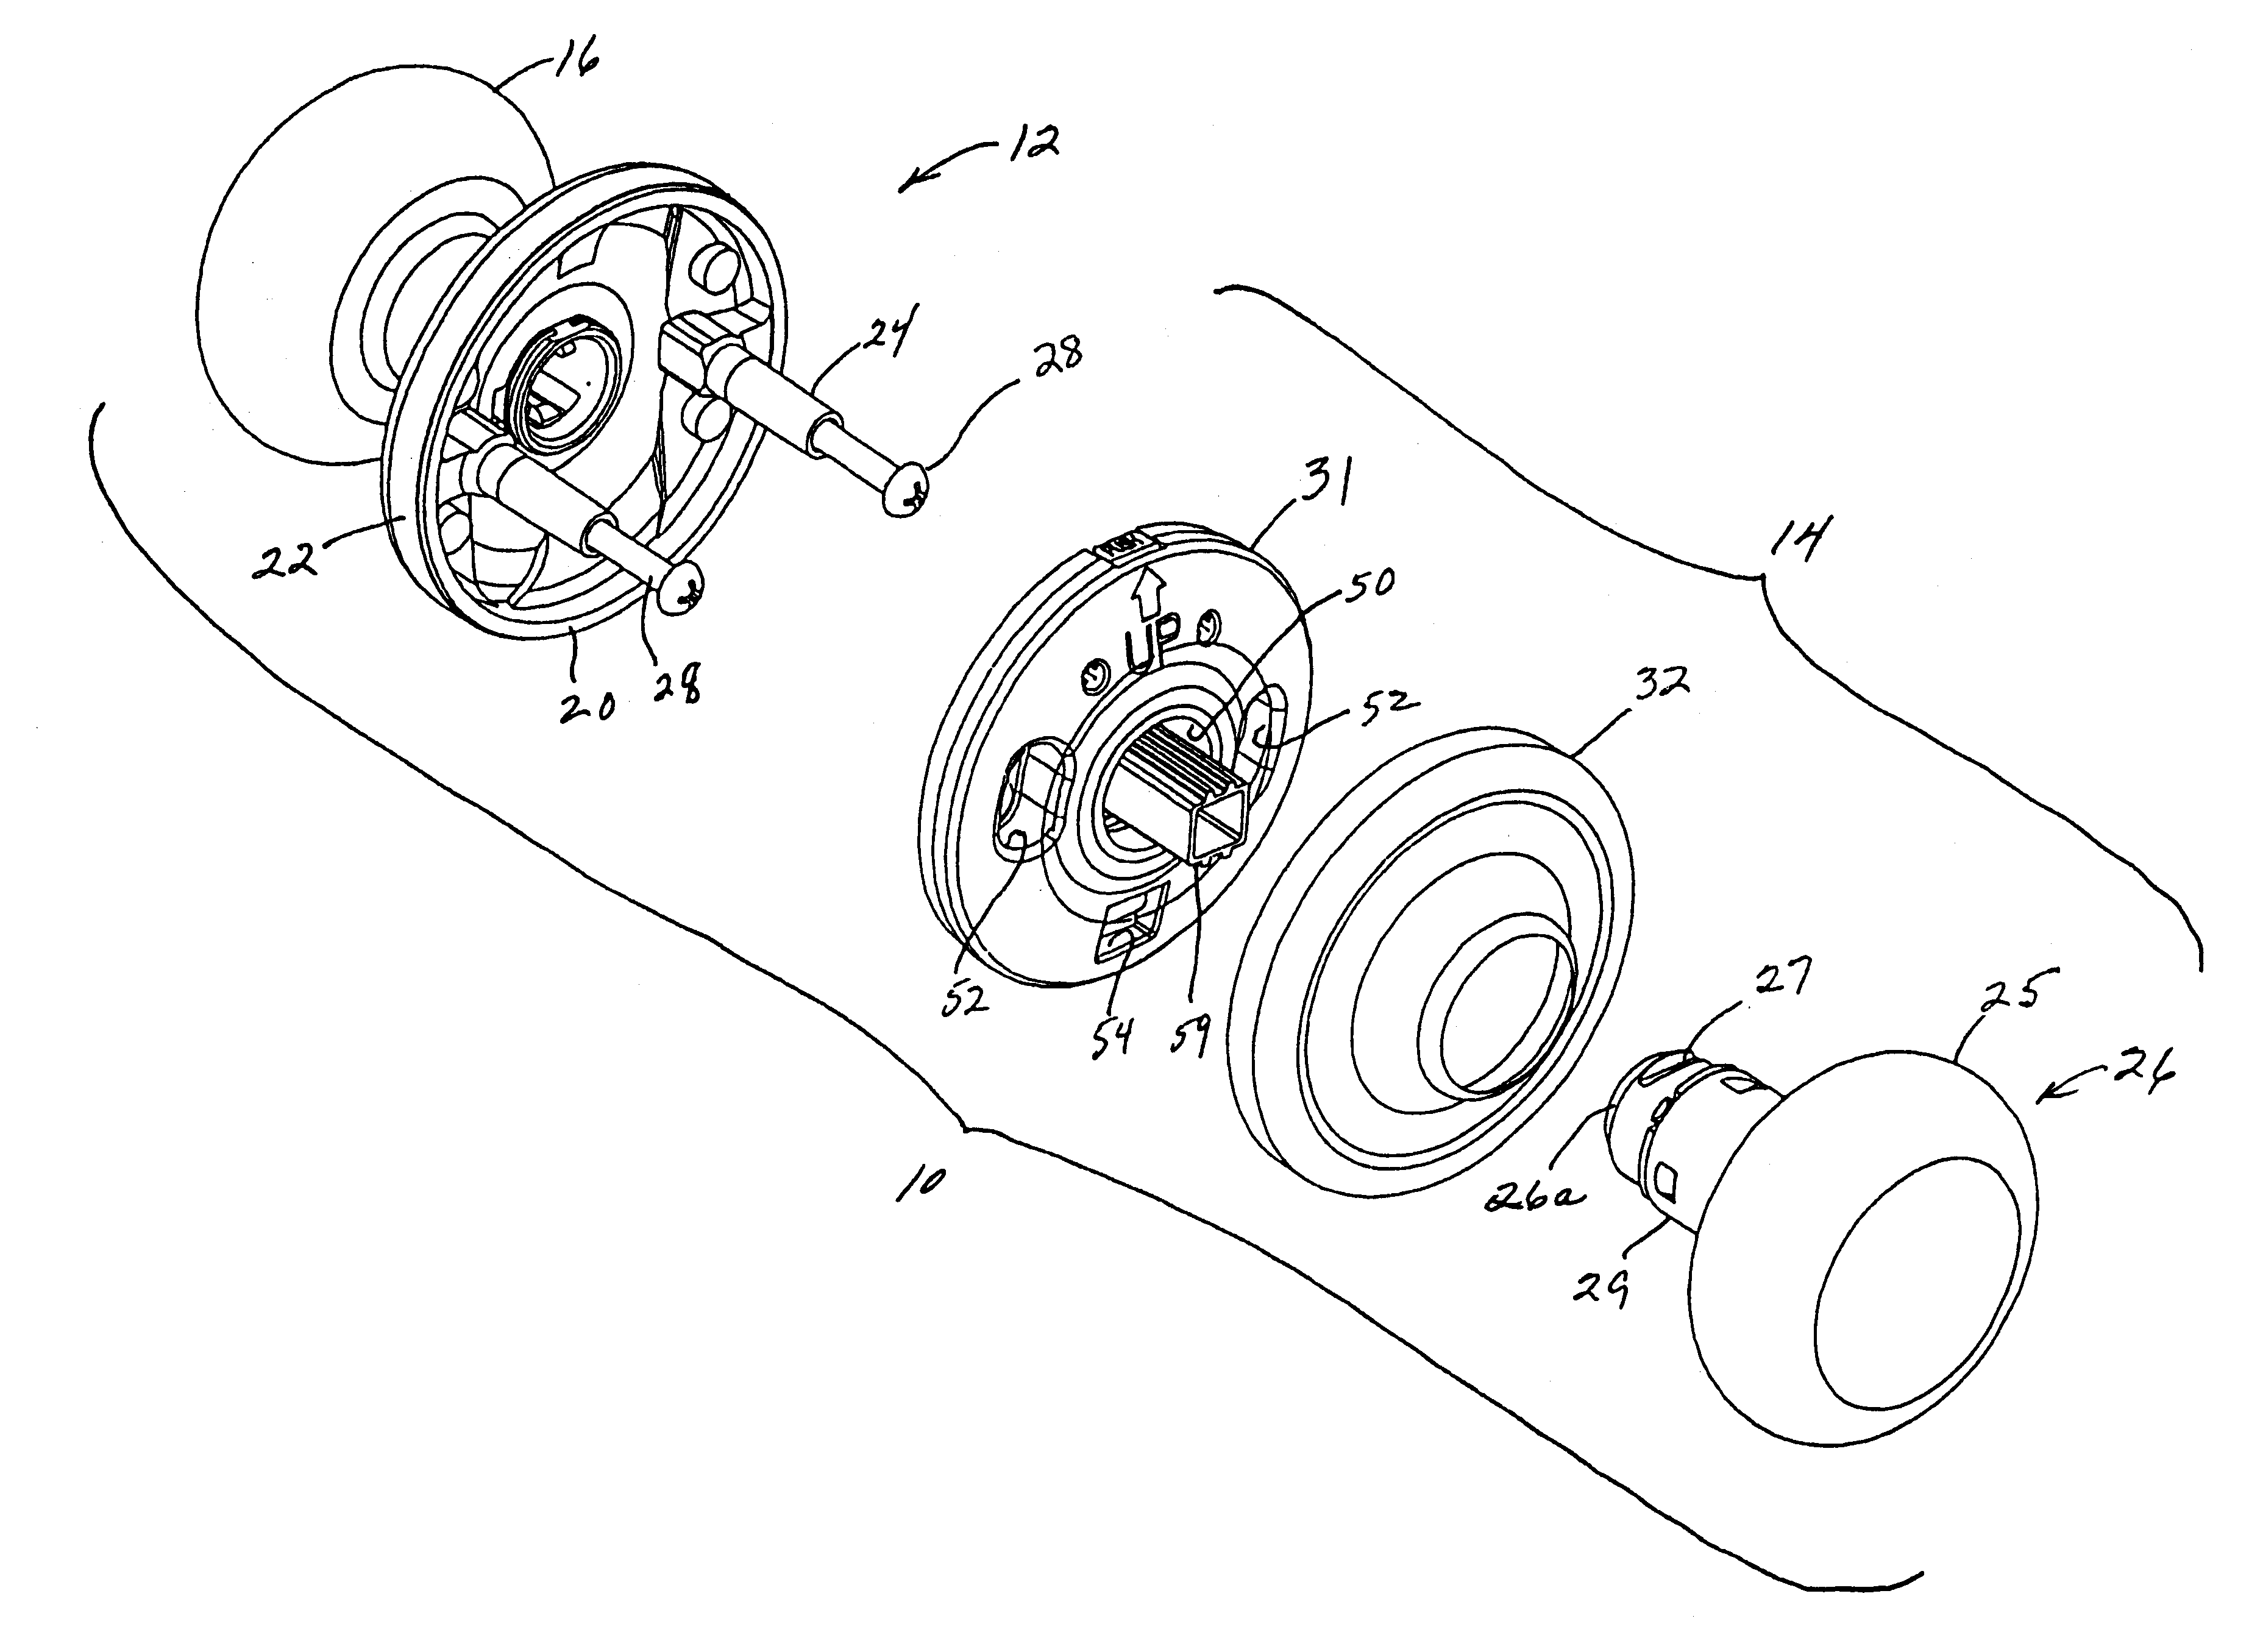
\includegraphics[scale=0.04]{components}
    \end{column}
    \begin{column}[b]{5.5cm}
      \begin{itemize}
      \item[] custom allocator
      \item[] stack map emission
      \item[] stack crawler
      \item[] registry of global roots
      \item[] type map
      \item[] collector runtime
      \end{itemize}
    \end{column}
  \end{columns}
\end{frame}

\begin{frame}{three axes of work}
  \begin{center}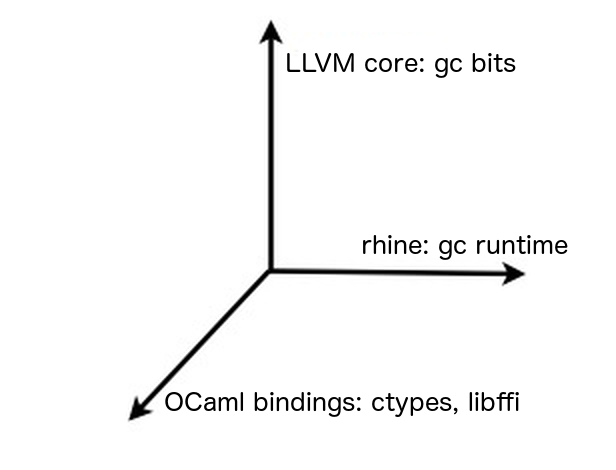
\includegraphics[scale=0.3]{xyz-axes}\end{center}
\end{frame}

\begin{frame}{current progress}
  \begin{tabular}{l r}
    llvm.git         & \texttt{ced3d1}, \texttt{79e72d} \\
    rhine.git        & \texttt{69a6f5..} \\
    ocaml-ctypes.git & \texttt{\#220} \\
  \end{tabular}
\end{frame}

\begin{frame}{end notes}
  \begin{enumerate}
  \item http://llvm.org/docs/GarbageCollection.html
  \item http://llvm.org/docs/LangRef.html
  \item \#ocaml on Freenode IRC
  \item \#llvm on OFTC IRC
  \end{enumerate}
\end{frame}

\end{document}

%%% Local Variables:
%%% mode: latex
%%% TeX-master: t
%%% End:
